% ==============================================================================
% CHAPTER 6: ARCHITECTURE-SELECTION GUIDE FOR MULTI-AGENT QA
% ==============================================================================
\section{Architecture-Selection Guide for Multi-Agent QA Systems}
\label{sec:guideline}

The preceding sections have systematically surveyed three architecture
classes and nine sub-paradigms of multi-agent collaborative QA systems
and have deeply examined the underlying enabling technologies of
communication, memory, and reasoning.
However, for practitioners the crux of architecture selection lies in
making an evidence-based decision among the many paradigms when faced with
a concrete application requirement.
Blindly adopting multi-agent collaboration not only fails to guarantee
gains; it can trigger coordination redundancy, cost explosion, and even
performance regression due to task--architecture mismatch.
The MAST failure taxonomy \citep{han2024mast} identifies recurring failures
in system design, inter-agent alignment, and task verification across more
than 1,600 annotated traces. These findings show that orchestration choices
can create failure modes even when the underlying models are capable.
This section provides researchers and engineers with a systematic and
actionable architecture-selection methodology to bridge the gap between
theoretical survey and engineering practice.

% ── 6.1  Methodological Foundation: DSRM ──────────────────────────────────────
\subsection{Methodological Foundation: DSRM}
\label{sec:dsrm}

The architecture-selection guide presented in this chapter is not derived
from subjective experience alone; it is built through theory-driven
deduction following the \textbf{Design Science Research Methodology (DSRM)}
\citep{peffers2007dsrm}, an established framework in information-systems
research for constructing and evaluating design artifacts (e.g., frameworks,
models, and methods).
DSRM's canonical six-step process maps precisely to the logic and
validation cycle of this chapter:

\begin{enumerate}
  \item \textbf{Problem identification and motivation}: Blind adoption of
    multi-agent technology can be catastrophic; practitioners urgently need
    a solution to the real-world pain point of ``which architecture to select
    for a given application scenario.''
  \item \textbf{Define objectives of a solution}: Construct a logically
    clear, qualitatively operable selection decision tree that lowers the
    trial-and-error cost and decision threshold of architecture design.
  \item \textbf{Design and development}: Based on the theoretical survey of
    multi-agent architecture paradigms and mechanisms in Chapters~2--4,
    extract three ``key decision factors'' influencing selection, and then
    deduce a ``two-phase architecture decision flow.''
  \item \textbf{Demonstration}: Apply the decision flow to five representative
    application scenarios (healthcare, legal, software engineering, etc.),
    demonstrating the rationality and usability of the reasoning logic.
  \item \textbf{Evaluation}: This chapter applies the decision factors to 10
    multi-agent systems relevant to QA and the reviewed domains, and compares the inferred
    architecture with the architecture adopted by the original authors. This
    diagnostic stress test examines the framework's consistency and identifies
    boundary cases without claiming general external validity.
  \item \textbf{Communication}: Systematically distill the complete loop from
    theory to practice into this survey chapter as a methodological reference
    for academia and industry.
\end{enumerate}

By organizing the guide around DSRM stages, this chapter re-frames the
system-level architecture-design problem---which has heavily relied on
expert intuition---as a transparent, theory-informed decision process. The
subsequent ten-case stress test probes internal consistency and boundary cases;
it is not a claim of independent external validation.

% ── 6.2  Core Principles ──────────────────────────────────────────────────────
\subsection{Core Principles of Architecture Selection}
\label{sec:principles}

Architecture selection should avoid technology trend-chasing and instead
be grounded in a deep understanding of scenario characteristics.
Three core principles underpin this framework:

\textbf{(1) Task-Driven}: The primary starting point for architecture
selection is an objective assessment of the target task's characteristics.
Every architecture decision should proceed from ``what are the features of
the QA task in this scenario?'' rather than from a subjective preference
for a specific technology.

\textbf{(2) Cost-Aware}: Introducing multi-agent collaboration inevitably
entails higher system complexity, communication overhead (token consumption),
and inference latency.
Only when the quality gains from multi-agent collaboration can sufficiently
offset these costs does a collaborative architecture hold practical value
\citep{han2024mast}.

\textbf{(3) Risk-Sensitive}: In high-stakes decision domains such as
healthcare, legal, and finance, safety and explainability requirements far
outweigh the pursuit of execution efficiency.
Such scenarios require not only rigorous architecture design, but also
embedded Human-in-the-Loop (HITL) intervention mechanisms.

% ── 6.3  Key Decision Factors ─────────────────────────────────────────────────
\subsection{Key Decision Factors}
\label{sec:decision_factors}

Three core dimensions drive the architecture decision---hereinafter called
``Key Decision Factors''.
They directly determine whether the system needs multiple agents, what
topology is required, and whether human intervention is necessary.

\textbf{1.\ Task Complexity and Domain Span.}
This is the primary condition for determining ``whether multiple agents are
needed.''
If the task is a single-step factual query with simple logic (e.g., weather
lookup, simple chitchat), the model's internal knowledge is sufficient and
a single-agent solution enjoys an absolute advantage in latency and cost.
However, when the task involves multi-step reasoning or spans multiple
specialized sub-fields (e.g., a combined consultation involving internal
medicine, surgery, and pharmacy, or a software-engineering closed loop
encompassing product, development, and testing), a single model is prone
to knowledge gaps and hallucination, triggering the need for multi-role
specialization and collaboration.

\textbf{2.\ Process Standardization and Dynamism.}
This determines ``what topology the system should adopt.''
If the task has a clear standard operating procedure (SOP)---such as
enterprise research report generation or code compilation debugging---where
processing steps exhibit strict serial dependencies, this strongly
suits a \textbf{Hierarchical} or pipeline architecture.
Conversely, if the problem is open-ended with no standard answer and
requires multi-perspective divergent collision (e.g., scientific hypothesis
exploration, open-domain knowledge debate), a \textbf{Flat} peer
architecture is more appropriate.
If task difficulty fluctuates greatly---mixing routine answers with
occasional deep complex logic---an \textbf{Hybrid} architecture capable
of adaptive scheduling is needed.

\textbf{3.\ Risk Tolerance and Audibility Requirements.}
The tolerable error rate of output results directly affects the system's
decision-authority boundary.
For chitchat, literary creation, or brainstorming, minor imperfections
are acceptable.
But for legal verdict prediction or medical prescription generation,
not only is hallucination ``zero-tolerable,'' but every reasoning step
must have a traceable legal or pathological basis.
In low-tolerance, high-risk domains, the system must adopt an architecture
that contains HITL nodes, using LLMs for high-concurrency background
analysis while reserving final adjudication authority for human experts.

% ── 6.4  Two-Phase Decision Flow ──────────────────────────────────────────────
\subsection{Two-Phase Architecture Decision Flow}
\label{sec:two_phase}

Based on the three Key Decision Factors above, this paper constructs the
two-phase architecture decision flow shown in Fig.~\ref{fig:decision_flow},
intended to provide heuristic-driven decision guidance.

\textbf{Phase 1 (Pre-screening)}: This phase aims to rapidly filter out
extreme scenarios.
Task complexity is considered first: if the task logic is simple and
requires no cross-domain knowledge, a single-agent approach should be
preferred to control costs.
Safety risk is then assessed: if the target scenario is in a
strictly regulated, zero-error-tolerance domain such as healthcare or
law, the safety-risk factor immediately routes the system to a
\textbf{Hybrid + HITL} architecture with a safety backstop, bypassing
all purely automated paradigms.

\textbf{Phase 2 (Fine-selection)}: For ordinary medium-to-high complexity
scenarios that pass pre-screening, the framework further deduces from the
degree of process standardization and dynamic divergence.
High process standardization points to \textbf{Hierarchical}; extreme
variability in task difficulty points to \textbf{Hybrid}; emphasis on
free divergence and multi-perspective verification points to \textbf{Flat}.

\begin{figure*}[pos=t]
  \centering
  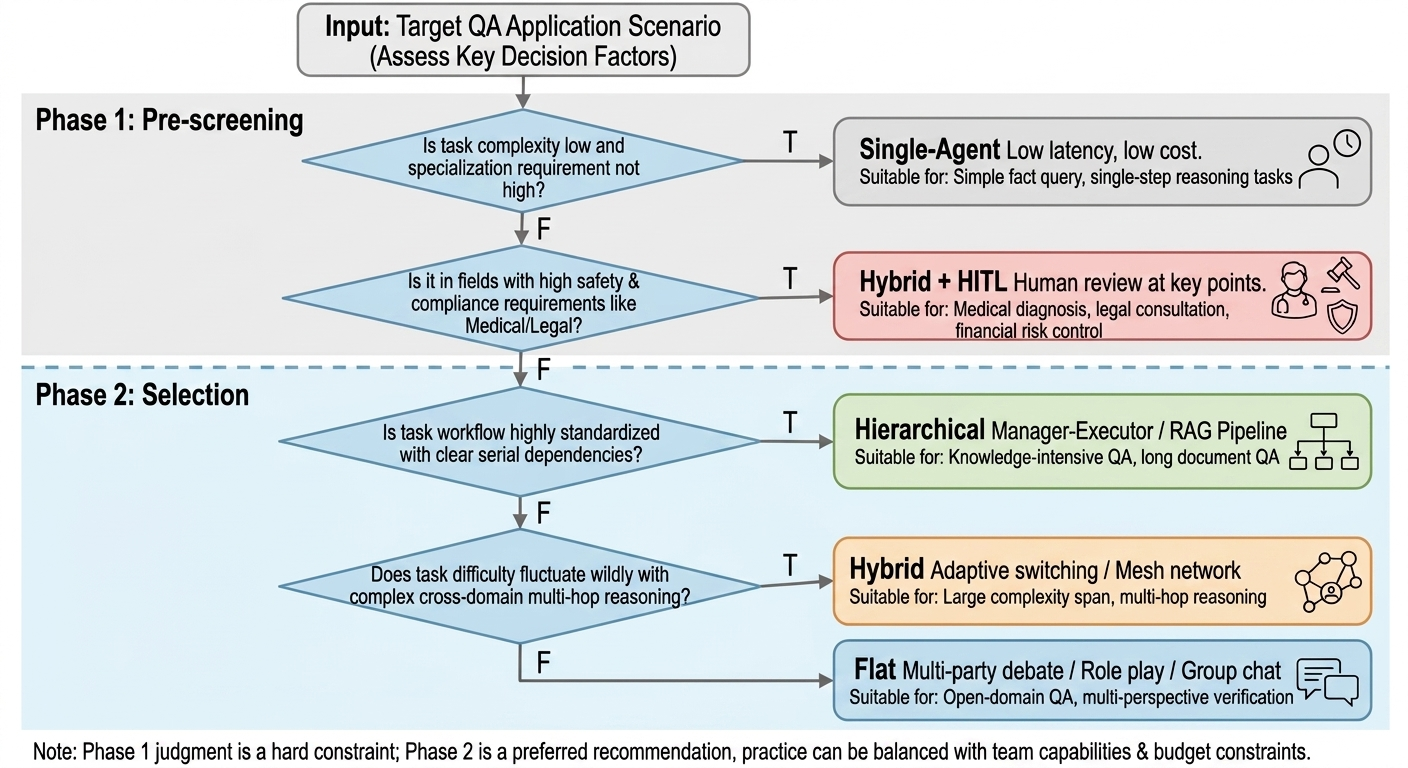
\includegraphics[width=\linewidth]{fig_flow.jpg}
  \caption{Two-phase decision flowchart for multi-agent QA architecture
           selection across application scenarios.}
  \label{fig:decision_flow}
\end{figure*}

% ── 6.5  Scenario Case Studies ────────────────────────────────────────────────
\subsection{Typical Scenario Case Studies}
\label{sec:case_studies}

To demonstrate the practical application of the qualitative decision
framework, five representative QA application scenarios are reasoned through.

\subsubsection{Scenario 1: Hospital Public Health Consultation}

\textbf{Profile}: Symptom analysis and triage guidance for the general
public, requiring knowledge spanning internal medicine, surgery, and
pharmacy, with extremely high demands for factual accuracy.

\textbf{Reasoning}: The scenario spans multiple medical specialties with
a vast knowledge domain, making single-model hallucination highly likely
and triggering the need for multi-agent expert consultation.
The extremely high medical safety risk and liability requirements mean that
the system must not operate in a fully closed-loop autonomous manner.
The safety-risk factor in Phase 1 directly eliminates purely automated
paths, strongly routing to a \textbf{Hybrid + HITL} architecture: lower
layers consist of multiple specialised agents debating in parallel, while
the top layer has human physicians performing final prescription and
diagnostic review.
MDAgents \citep{kim2024mdagents} illustrates this multi-specialty role
collaboration with safety review in analogous scenarios.

\subsubsection{Scenario 2: Enterprise Internal Knowledge-Base QA}

\textbf{Profile}: Precise QA for large-enterprise employees based on vast
policy documents and product manuals, where every answer must have a
traceable document source.

\textbf{Reasoning}: The scenario features highly standardized business
processes, linear logic, and answers fully converging on existing
documents, with no need for excessive creative divergence.
The high Process Standardization characteristic strongly suits a
\textbf{Hierarchical RAG Pipeline}: a rigid processing chain of
``Planner $\to$ Retriever $\to$ Generator $\to$ Verifier'' ensures reliable
information transmission.
LONGAGENT \citep{zhao2024longagent} demonstrates the efficiency and
rigor of this serial pipeline in ultra-long document QA.

\subsubsection{Scenario 3: Online Education Open-Domain QA}

\textbf{Profile}: Cross-disciplinary QA for students (mathematics, physics,
literature); the system must not only provide correct answers but must
heuristically guide students to think actively.

\textbf{Reasoning}: The questions are highly open-ended and divergent with
no fixed pipeline steps and relatively low safety risk.
To achieve heuristic teaching, the system needs multi-perspective viewpoints
and dialectical problem-solving.
This characteristic points to a \textbf{Flat} architecture.
Constructing a role-based group chat or debate (e.g., tutor, corrector,
knowledge extender) simulates classroom brainstorming, consistent with the
designs of CAMEL \citep{li2023camel} and debate mechanisms
\citep{du2024multiagent_debate}.

\subsubsection{Scenario 4: Legal Document Retrieval and Consultation}

\textbf{Profile}: Assisting lawyers with contract review and sentencing
prediction; involves lengthy legal document comparison, extremely rigorous
logical deduction, and outputs with legal reference value.

\textbf{Reasoning}: Legal statute comparison demands a rigorous retrieval
engine (pointing to a hierarchical retrieval base), while case characterization
and sentencing require multi-angle legal discourse (calling for a flat debate
mechanism), and the high cost of legal errors requires a human lawyer to
intervene at the final node.
The superposition of these three characteristics makes this scenario
a textbook example of a \textbf{Hybrid} architecture: a backbone of
``Hierarchical RAG + Flat Debate Enhancement + Human Review Backstop'' that
balances deep retrieval with prudent decision-making \citep{gao2024rag_survey}.

\subsubsection{Scenario 5: Software Engineering QA and Code Generation}

\textbf{Profile}: Code generation, bug analysis, and automated testing for
R\&D teams; clear input--output specifications and unambiguous evaluation
criteria (whether code compiles successfully).

\textbf{Reasoning}: Software engineering is inherently highly process-
standardised; every step from requirements to design, coding, and testing
depends strictly on the output of the preceding node.
This ``waterfall''-style industrial production mode directly corresponds to
the \textbf{Hierarchical Manager--Executor} pattern.
MetaGPT \citep{hong2024metagpt} and ChatDev \citep{qian2023chatdev} provide
representative implementations of this manager--executor logic, supporting
its plausibility without independently validating the selection framework.

% ── 6.6  External Validation ──────────────────────────────────────────────────
\subsection{Architecture-Selection Stress Test}
\label{sec:validation}

To examine the diagnostic utility and boundary conditions of the selection
framework, this section adopts a consistent deduction--comparison procedure.
Ten published multi-agent systems relevant to QA and the reviewed application
domains are selected under
the following four criteria.
(1)~\textbf{Publication window and venue}: papers published between 2022 and
2026, consistent with the survey retrieval window, sourced from peer-reviewed
venues including ACL, EMNLP, ICML, IEEE Transactions, and ACM conferences,
with one arXiv preprint included to cover code generation.
(2)~\textbf{Structural transparency}: each paper must explicitly describe
the agent roles, collaboration topology, and design rationale of its system,
providing sufficient detail for a principled architecture comparison.
(3)~\textbf{Task diversity}: the cases cover tasks with different levels of
openness, process standardisation, domain specialisation, and deployment risk.
(4)~\textbf{Purposive coverage}: the sample covers
the major application domains reviewed in Section~5 (healthcare $\times$2,
legal $\times$1, software engineering $\times$2, education $\times$1,
finance $\times$1, and general/enterprise QA $\times$3).
Each paper's application scenario is coded using the same three Key Decision
Factors, and a recommended architecture is inferred and compared with the
architecture adopted by the original authors, as shown in
Table~\ref{tab:validation}.

The comparison yields five broadly aligned cases, three partially aligned
cases, and two divergent cases. LegalGraphRAG, Triad, LONGAGENT, ChatDev, and
AgentCoder broadly follow the architecture inferred from their task profiles.
MedAgents and LLM-MedQA preserve parallel expert perspectives but add staged
synthesis and decision components, so they are better described as hybrid
workflows than as purely flat voting systems. MAD
\citep{du2024multiagent_debate} is flat at the macro level, although its
iterative convergence procedure is not the explicit vote round anticipated
by the decision guide. EduPlanner \citep{zhang2024eduplanner} and Financial
Reflection QA \citep{fatemi2024financialqa} are divergent cases: both combine
an apparently convergent task objective with iterative evaluator/critic
feedback. These cases expose the limitation of treating one task dimension
as dominant. The comparison is an author-coded diagnostic exercise, not an
independent statistical validation of the framework.

\begin{table*}[pos=t]
  \centering
  \caption{Diagnostic stress test of the architecture-selection framework
           using 10 vertical-domain papers.}
  \label{tab:validation}
  \small
  \resizebox{\linewidth}{!}{%
  \begin{tabular}{p{2.2cm} p{2.6cm} p{4.8cm} p{2.4cm} p{3.4cm} c}
    \toprule
    \textbf{System} & \textbf{Application} &
    \textbf{Key Decision-Factor Profile} &
    \textbf{Inferred Arch.} & \textbf{Actual Arch.} &
    \textbf{Match} \\
    \midrule
    MedAgents \citep{tang2024medagents} &
      Multi-specialty medical QA &
      Cross-specialty high complexity; non-standardisable reasoning; moderate risk &
      Flat (multi-role collaboration) &
      Hybrid (parallel expert analyses + staged synthesis and decision) & $\triangle$ \\[3pt]
    LLM-MedQA \citep{tang2025llmmedqa} &
      Standardised medical MCQ &
      Moderate complexity; convergent objective but divergent perspectives; moderate risk &
      Flat (multi-view + vote aggregation) &
      Hybrid (question/option experts + six-stage voting and decision pipeline) & $\triangle$ \\[3pt]
    LegalGraphRAG \citep{legalgraphrag2026} &
      Legal verdict prediction &
      Multi-level legal reasoning; standardised retrieval + open reasoning; zero-tolerance high risk &
      Hybrid (hierarchical RAG + flat review) &
      Hybrid (layered graph + three-role audit chain) & \checkmark \\[3pt]
    Triad \citep{hu2024triad} &
      Enterprise structured KBQA &
      Moderate complexity; Text-to-SPARQL highly standardised; moderate risk &
      Hierarchical (rigid pipeline) &
      Hierarchical (three-role four-stage serial pipeline) & \checkmark \\[3pt]
    LONGAGENT \citep{zhao2024longagent} &
      Ultra-long document multi-hop QA &
      High complexity; divide-and-conquer SOP; moderate risk &
      Hierarchical (Leader--Member) &
      Hierarchical (Leader dispatch + Member parallel) & \checkmark \\[3pt]
    ChatDev \citep{qian2023chatdev} &
      Full-cycle software engineering &
      High complexity; very high waterfall standardisation; moderate risk &
      Hierarchical (waterfall pipeline) &
      Hierarchical (multi-role Chat Chain serial pipeline) & \checkmark \\[3pt]
    AgentCoder \citep{huang2023agentcoder} &
      Code generation and iterative testing &
      Moderate complexity; clear three-role data-flow dependency; low risk &
      Hierarchical (rigid three-role pipeline) &
      Hierarchical (coder $\to$ test-designer $\to$ executor + feedback loop) & \checkmark \\[3pt]
    MAD \citep{du2024multiagent_debate} &
      Open-domain factual \& maths reasoning &
      High openness; no standard workflow; low risk &
      Flat (multi-view debate + vote convergence) &
      Flat (peer debate + iterative convergence, no explicit vote round) & $\triangle$ \\[3pt]
    EduPlanner \citep{zhang2024eduplanner} &
      Adaptive educational planning &
      Open education + convergent curriculum-scoring objective; dual features; low risk &
      Flat (multi-view discussion) &
      Hierarchical (Evaluator--Optimizer adversarial pipeline) & $\times$ \\[3pt]
    Financial Reflection QA \citep{fatemi2024financialqa} &
      Financial numerical reasoning QA &
      Convergent target + reasoning requires self-critique; dual features; moderate risk &
      Hierarchical (RAG pipeline) &
      Hybrid (Solver + multi-Critic reflection loop) & $\times$ \\
    \bottomrule
  \end{tabular}}
  \footnotesize
  \textit{Note}: \checkmark = broadly aligned; $\triangle$ = partially
  aligned but with an additional coordination layer or different convergence
  mechanism; $\times$ = divergent inferred and implemented architecture.
  The labels are diagnostic author coding rather than independent validation.
\end{table*}

The five aligned, three partial, and two divergent cases should not be read as
a performance estimate. Instead, they show where the guide is diagnostically
useful and where staged synthesis or critic feedback makes a single-label
classification ambiguous. The divergent cases occur in boundary scenarios
with competing task requirements, indicating that the framework is more
decisive when one requirement dominates and less decisive when several
dimensions pull the design towards different architectures.

% ── 6.7  Limitations ──────────────────────────────────────────────────────────
\subsection{Summary and Limitations}
\label{sec:limitations}

This chapter transcends conventional technology enumeration and constructs
a complete architecture-selection methodology---comprising key decision
factor extraction, a two-phase decision flowchart
(Fig.~\ref{fig:decision_flow}), and scenario case studies---grounded in
three core principles: task-driven, cost-aware, and risk-sensitive.
This system transforms what has been a highly expert-intuition-dependent
architecture design problem into a qualitatively decomposable, systematic
decision process for researchers and engineers facing multi-agent technology
choices.

The following limitations are acknowledged.
\textbf{(1) Competing-requirement ambiguity}: as demonstrated by the stress test,
when a task simultaneously possesses competing open-ended and standardised
features, the framework's single-dimension deduction is prone to error;
a priority-weighting mechanism is needed.
\textbf{(2) Temporal validity}: cutting-edge multi-agent technologies
(e.g., dynamic routing algorithms, adaptive role switching) are still
evolving rapidly; some boundary-clear recommendations in the framework
may converge in the future.
\textbf{(3) Limited stress-test scale}: the ten purposively selected systems
form a local diagnostic sample, so external validity awaits larger-scale,
pre-registered testing on independently sampled systems.
